\title{Nebenläufigkeit bei Betriebssystemen}
\subtitle{Ein Überblick}

\author{Arne Struck}

\institute{Universität Hamburg\\ 
  Fakultät für Mathematik, Informatik und Naturwissenschaften\\
  Fachbereich Informatik, Arbeitsbereich TGI\\
  Proseminar Nebenläufigkeit SS 14}
  
\date{\today}

\maketitle

\index{personen}{Struck, Arne}

%\markboth{\textit{Nebenläufigkeit SS\/14}: Struck} Sieht ein wenig komisch aus, so am Zeilenkopf
%{Nebenläufigkeit bei Betriebssystemen}
\begin{abstract}
Diese Arbeit soll einen Überblick über die Verteilung der Systemressourcen (insbesondere der CPU) an 
verschiedene Prozesse und somit deren Möglichkeiten zur Nebenläufigkeit verschaffen. Dazu werden Strategien 
zur Verteilung und einige der vorkommenden Probleme dieser beleuchtet. Dies wird für die drei Bereiche der 
Stacksysteme, der interaktiven Systeme (wobei hier der Schwerpunkt liegt) und der Echtzeitsysteme 
geschehen. Auf dieser Basis wird im folgenden Multiprozessor-Systeme behandelt, wobei erst einmal der 
Aufbau erläutert und dann auf das Scheduling eingegangen wird. 
\keywords{Scheduling, Multiprozessor-Scheduling, Synchronisation, Echtzeitsysteme}
\end{abstract}

\tableofcontents
\newpage

\section{Einleitung}
Sobald ein Rechner(system) dazu fähig ist mehr als eine bestimmte Aufgabe auszuführen, können diese 
Aufgaben in Form von Prozessen und Threads beginnen miteinander um die Systemressourcen zu konkurrieren.
Im folgenden werden Threads implizit behandelt, da für sie als leichtgewichtige Prozesse ähnliche 
Prinzipien gelten. \\
Der Konkurrenzfall tritt ein, sobald zwei Prozesse zu sich überschneidenden Zeiten rechenbereit sind. Falls 
nicht ausreichend Ressourcen oder Softwaretechnische Mittel existieren, damit die Prozesse eine zeitgleiche 
Ausführung erlaubt ist, müssen die Ressourcen aufgeteilt werden. Diese Aufteilung nennt sich Scheduling und 
ist heutzutage besonders im Falle der Rechenzeit einer CPU relevant, da sie bei einem Rechner das 
bestimmende Element ist. Das Verfahren nachdem die Ressourcen aufgeteilt werden wird als Scheduling-
Strategie bezeichnet. \\

\section{Scheduling - allgemeines}
Das allgemeine Ziel von Scheduling sollte sich von selbst erschließen, die Systemressourcen möglichst 
optimal auszulasten (Balance), aber gleichzeitig keinen Prozess zu benachteiligen (Fairness) wobei zwar je 
nach Fall sowohl das eine, als auch das andere korrekt sein kann, ist in den meisten Anwendungen letzteres 
das wichtigere. Es wäre beispielsweise durchaus problematisch, sollten in einem Automobil die Kontrolle der 
Lichtanlage und der Bremsen durch den selben Mikrocontroller bearbeitet werden und die Lichtanlage vom 
Scheduler immer eine höhere Priorität eingeräumt bekommen. \\
Aber natürlich hat jedes System auch seine eigenen Scheduling-Ziele: \\ \\
\textbf{Stacksysteme}
\begin{itemize}
	\item Maximierung des Durchsatzes (der geleisteten Arbeit)
	\item Minimierung der Durchlaufzeit
	\item Maximierung der CPU-Auslastung
\end{itemize}
\textbf{Interaktive Systeme}
\begin{itemize}
	\item Reduktion der Antwortzeit
	\item Proportionalität gewährleisten (Benutzererwartung erfüllen)
\end{itemize}
\textbf{Echtzeitsysteme}
\begin{itemize}
	\item Deadlines einhalten
	\item Vorhersagbarkeit (Reduktion des Qualitätsverlustes in Multimedia-Systemen)
\end{itemize}
\cite{tanenb2009} \\ \\
Scheduling-Strategien müssen diese Ziele mit ihrer Strategie vereinigen und dadurch ein akzeptables 
Scheduling erzeugen. \\
Aber wann muss Scheduling erfolgen? Hier existieren Standartfälle, welche überall vorkommen können und 
besondere Fälle, welche von der durchzusetzenden Strategie und dem System an sich abhängen. Beispiele für 
diese Standartfälle wären die Entscheidung ob bei frischem Spawn Eltern- oder Kindprozess weiterlaufen 
dürfen und die Entscheidung welcher Prozess weiter bearbeitet wird, sollte ein Prozess terminieren oder 
blockiert (zum Beispiel durch eine Ein- oder Ausgabeanfrage). \\
Scheduling-Strategien können verdrängend oder nicht verdrängend sein. Nicht verdrängend bedeutet, dass 
sobald ein Prozess die Priorität bekommt, rechnet er bis zur Blockierung oder Terminierung. Verdrängend 
wiederum beschreibt die Eigenschaft einer Strategie einen Prozess in seiner Ausführung vom Scheduler 
unterbrechbar zu machen, sollte ein Prozess mit nach der Scheduling Strategie stärkeren Priorität in der 
Menge der zu bearbeitenden Prozesse erscheinen. Der verdrängte Prozess wird der Menge zugeschlagen.
\\
%stack
\section{verschiedene Strategien}
\subsection{First Come, First Serve}
Die First Come, First Serve Strategie ist die simpelste Idee für ein Scheduling und findet auch in anderen 
Bereichen der Informatik Anwendung. Es handelt sich hierbei um eine nicht verdrängende Strategie.
Das Verfahren ist einfach zusammenzufassen: Der erste Prozess, welcher Rechenbereitschaft meldet bekommt 
die Systemressourcen, der zweite Prozess, welcher Rechenbereitschaft meldet bekommt den ersten Platz in der 
Warteschlange, der Dritte den zweiten Platz und so weiter. \\
Dies macht die Strategie einfach zu implementieren und der findige Leser hat auch schon den Vorschlag 
herauslesen können. \\
Ein Beispielscheduling, die grau eingefärbten Blöcke beschreiben die Rechenzeit des Auftrags, während die 
schraffierten Blöcke Prozesswechselzeit markieren. \\ \\
\begin{center}
\begin{tabular}{l|c|c|c|c|c}
	Auftrag               & \(A_1\)  & \(A_2\)  & \(A_3\) & \(A_4\) & \(A_5\) \\ \hline \hline
	Ankunftszeit		  & 1        &  5		& 4       & 8       &  2      \\ \hline
	Bedienzeitanforderung & 3        &  4       & 2       & 6       &  3      \\
\end{tabular}
\end{center}
\begin{center}
\begin{blockgraph}{25}{1}{0.4}
    \bglabelxx{0}
    \bglabelxx{5}
    \bglabelxx{10}
    \bglabelxx{15}
    \bglabelxx{20}
	\bglabelxx{25}
   
   	\bgblock{0}{3}{$A_1$}
   	\bgemptyblock{3}{4}
   	\bgblock{4}{7}{$A_5$}
   	\bgemptyblock{7}{8}
   	\bgblock{8}{10}{$A_3$}
   	\bgemptyblock{10}{11}
   	\bgblock{11}{15}{$A_2$}
   	\bgemptyblock{15}{16}
   	\bgblock{16}{22}{$A_4$}
\end{blockgraph}
\end{center}

\subsection{Shortest Job First}
Bei dieser nicht verdrängenden Strategie wird aus der Menge, der zur Ausführung stehenden Prozessen 
derjenige mit der geringsten Ausführungszeit gewählt. Dies setzt voraus, dass die zu erwartenden 
Ausführungszeiten bekannt sind. Dies ist auf zwei Arten realistisch zu erreichen: das Programm wurde vom 
Entwickler auf Laufzeiten getestet, diese müssen dann von allen Entwicklern norminalisiert werden und 
stellt die Information bereit. Dies ist im großen Rahmen nicht praktikabel. Oder es handelt sich um immer 
wiederkehrende Prozesse, dann kann der Scheduler über statistische Verfahren eine ungefähre Laufzeit 
abschätzen. \\
Allerdings beinhaltet er die Schwachstelle, dass es sich um eine unfaire Strategie handelt, sobald ein 
Prozessspawn existiert. Dies lässt sich an folgendem Minimalbeispiel nachvollziehen: \\
Gegeben seien drei Prozesse A, B und C, Prozess A und B haben eine zu erwartende Ausführungszeit von 1 und 
2 Prozess C von 20. Nun wird zu erst A, dann B abgearbeitet. Sollte nun in der Abarbeitungszeit von B ein 
neuer Prozess A durch B gespawnt werden, wird dieser in die Menge der zu bearbeitenden Prozesse 
aufgenommen. Sollte nun dieser neue Prozess A einen neuen Prozess B spawnen, befinden wir uns in einer 
endlosen Schleife, welche die Bearbeitung von C nicht erlaubt.
Was den Datendurchsatz angeht ist diese Strategie nachweislich optimal \cite{tanenb2009}


\subsection{Shortest Remaining Time Next}
Bei Shortest Remaining Time Next handelt es sich um eine verdrängende Adaption von Shortest Job First.  
Anstatt der Gesamtdauer des Prozesses, wird die noch verbleibende Ausführungszeit eines Prozesses 
berücksichtigt, wobei bei einem frischen Prozess natürlich die komplette zu erwartende Ausführungszeit der 
verbleibenden entspricht. \\
Die löst einen großen Teil, der Fairness-Probleme, das Problem aus dem Minimalbeispiel bleibt jedoch 
bestehen. 

%interaktive Systeme
\subsection{Round Robin}
Das Round Robin Verfahren ist meist in interaktiven Systemen zu finden. Es handelt sich um eine durch das 
Verfahren bedingte verdrängende Strategie. Bei der Round Robin Strategie wird die CPU-Zeit in 
Zeitabschnitte unterteilt, wobei jeder Prozess einen Abschnitt zugeordnet bekommt. Nachdem dieser Abschnitt 
genutzt wurde, wird der Prozess ans Ende der Queue gesetzt. Sollte ein Zeitabschnitt durch Blockierung oder 
Terminierung nicht vollständig genutzt werden können, darf direkt der nächste rechenbereite Prozess 
beginnen. \\
Ein Problem des Round Robins ist die Annahme, dass alle Prozesse gleich zu priorisieren sind. Dies ist 
nicht immer der Fall, beispielsweise sollte eine gerade verwendete Echtzeitanforderung (beispielsweise ein 
Video) eine höhere Priorität genießen, als ein im Hintergrund geöffneter PDF-Reader. \\
Ein weiteres (aber durchaus lösbares) Problem ist die Wahl der Länge des Zeitabschnittes. Wird dieser zu 
lang gewählt, muss ein Prozess bei einer ausreichend großen Prozessmenge mehrere Sekunden warten. Man 
sollte diesen Zeitabschnitt allerdings auch nicht zu kurz wählen, da ein Prozesswechsel eine gewisse Zeit 
in Anspruch nimmt und der Anteil an Verwaltungszeit nicht zu hoch sein sollte. \\
Ein Beispielscheduling: \\ \\
\begin{center}
\begin{tabular}{l||c|c|c|c}
	Auftrag               & \(A_1\)  & \(A_2\)  & \(A_3\) & \(A_4\) \\ \hline \hline
	Ankunftszeit		  & 1        &  4		& 5       & 8       \\ \hline
	Bedienzeitanforderung & 6        &  4       & 2       & 6       \\
\end{tabular} \\ \quad \\
Zeitscheibengröße: \(\Delta t = 2\)
\end{center}
\begin{center}
\begin{blockgraph}{25}{1}{0.4}
    \bglabelxx{0}
    \bglabelxx{5}
    \bglabelxx{10}
    \bglabelxx{15}
    \bglabelxx{20}
	\bglabelxx{25}
   
   	\bgblock{0}{2}{$A_1$}
   	\bgblock{2}{4}{$A_1$}
   	\bgemptyblock{4}{5}
   	\bgblock{5}{7}{$A_2$}
   	\bgemptyblock{7}{8}
   	\bgblock{8}{10}{$A_1$}
   	\bgemptyblock{10}{11}
   	\bgblock{11}{13}{$A_3$}
   	\bgemptyblock{13}{14}
   	\bgblock{14}{16}{$A_2$}
   	\bgemptyblock{16}{17}
   	\bgblock{17}{19}{$A_4$}
   	\bgblock{19}{21}{$A_4$}
   	\bgblock{21}{23}{$A_4$}
\end{blockgraph}
\end{center}

\subsection{Priorisiertes Scheduling}
Das priorisierte Scheduling greift den Gedanken auf, dass unterschiedliche Prozesse unterschiedliche 
Prioritäten besitzen. Jeder Prozess bekommt sobald er Rechenbereitschaft meldet eine Priorität zugeordnet.
Diese wird nach den Einsatzbestimmungen des Systems vergeben. Sollte man Interaktivität wünschen, muss die 
Priorität während der Verarbeitung modifiziert werden, damit nicht der am höchsten priorisierte Prozess 
eine Verdrängung verhindert. \\
Eine Möglichkeit hierzu wäre beispielsweise das Herabsetzen der momentanen Priorität des rechnenden 
Prozesses bei jedem Taktzyklus, bis die Priorität nicht mehr die Höchste ist. Hierfür muss die 
Anfangspriorität ausreichend hoch gewählt werden, sodass bei langen Prozessen nicht eine Priorität von 0 
vorliegt. Alternativ könnte man die Priorität jedes rechenbereiten Prozesses jede nten Taktzyklus zu 
inkrementieren. \\
Die Prioritätsvergabe kann statisch oder dynamisch erfolgen. Ein Beispiel der statischen Vergabe wäre in 
einem Rechenzentrum, so könnten die Prozesse der Systemadministratoren eine Priorität von 100, die der 
Verwaltungsebene eine von 75 und die der User eine von 50 haben. \\
Eine dynamische Vergabe von Prioritäten ist bei der Berücksichtigung von Ein- und Ausgabeintensiven 
Prozessen interessant, da diese wenig Rechenzeit benötigen, aber aufgrund der im Vergleich langsamen 
Festplatten lange brauchen, bis sie erneut rechenbereit sind. Eine Realisierung wäre eine Priorität von 
\(\frac{1}{f}\) auf die Priorität aufzuschlagen, wobei \(f\) den Anteil der Nutzung des letzten dem Prozess 
zustehenden Zeitabschnittes darstellt. \\
Da für jeden Prozess Prioritäten zu managen einen relativ hohen Ressourcenverbrauch besitzt, ist es günstig 
Prioritätsklassen zu bilden und innerhalb dieser per Round Robin zu verfahren. \cite{OSThreePieces2014} \\
Ein Round Robin Zyklus würde einem Takt aus der nicht klassenbasierten Variante entsprechen. Eine andere 
Form würde das Abarbeiten der höchsten Prioritätsklasse und dann das der darauf folgenden Klasse, sobald 
die höchste Klasse leer ist. Natürlich müssen in diesem Verfahren die Klassen angepasst werden, damit 
Prozesse unterer Klassen nicht "verhungern". \cite{tanenb2009}

\subsection{Shortest Process Next}
Die Shortest Process Next Strategie ist der Versuch die Antwortzeiten der Shortest Job First Strategie in 
einem interaktiven System nutzbar zu machen. Die Information, welcher Prozess die kürzeste Laufzeit besitzt 
wird durch heuristische Verfahren auf Basis der bisherigen Ausführungen des Prozesses gewonnen. Bei immer 
wiederkehrenden Prozessen ist dies möglich, die Strategie hat durch die benötigte Profilierung der 
einzelnen Prozesse jedoch Probleme bei neuen, noch nicht profilierten Prozessen. \\
Abhilfe kann hier ein Profiling aller Programme des Systems verschaffen, dies ist effektiv nur für nicht 
veränderbare Systeme möglich. 

\subsection{Fair-Share-System}
Das Fair-Share-Scheduling-System stützt sich auf eine andere Definition von Fairness, es berücksichtigt den 
Besitzer der jeweiligen Prozesse. Wenn auf einem System mehrere Nutzer Prozesse laufen lassen, sollen also 
idealerweise \(\frac{1}{n}\) (wobei \(n\) der Anzahl der Nutzer entspricht) der CPU-Zeit pro Nutzer 
verwendet werden. \\
Ein Beispiel: Wenn Nutzer A einen Prozess auf einem System laufen lässt, Nutzer B allerdings 3, erhält 
Nutzer A bei einem Verfahren mit gleicher Priorisierung nur 25\% der Rechenzeit. \\
Eine mögliche, einfache Realisierung wäre hierbei das Einteilen der Prozesse in Klassen von Benutzern, 
wobei intern mit einem Scheduling freier Wahl verwendet werden kann und jedes Scheduling nach dem Round 
Robin Prinzip gleich lange CPU-Slots zugeteilt bekommt, diese Zeit-Slots werden in den einzelnen Klassen 
verarbeitet. Damit ein Nutzer nicht all zu lange auf seine Antworten warten muss, ist es möglich dass die 
Klassen an den Scheduler ihre Einteilungen vermitteln um somit dem Scheduler zu ermöglichen zwischen den 
Prozessen der unterschiedlichen Nutzer Abwechslung zu erzeugen.
\\

\section{Echtzeitscheduling}
Um bei Anwendungen mit relevanter Echtzeitkomponente ein Scheduling zu erreichen wird ein Programm in 
kleine, deterministische Prozesse unterteilt. Diese müssen nun durch den Scheduler so verteilt werden, dass 
sie die Zeitanforderungen des Anwendungsfalles erfüllen.

\subsection{Deadlines}
Bei Echtzeitsystemen spielt die Zeit in Form von Deadlines eine große Rolle. Deadlines werden in weiche und 
harte Deadlines unterteilt. Weiche Deadlines zeichnen sich durch eine verzeihliche Verletzungen aus, 
beispielsweise wenn ein Anwenderprogramm (zum Beispiel ein Videoplayer) sehr selten seine Deadline nicht 
einhält, dies führt zu einer leichten Verzögerung in der Ausgabe, nicht schön aber noch in vertretbaren 
Rahmen. Eine harte Deadline wäre der gegenteilige Fall. Ein Beispiel hierfür wäre die Robotik in der 
chirurgischen Medizin, sollten diese zu langsam reagieren (der Prozess also eine Antwort außerhalb der 
Deadline liefern) kann einem Patienten nachbleibende Schäden zugefügt werden. 

\subsection{Periodizität}
Zusätzlich werden die Prozesse in periodisch und aperiodisch unterteilt. Periodische Prozesse spawnen in 
bestimmten, regelmäßigen Abständen, aperiodische Prozesse hingegen spawnen in unterschiedlichen, nicht 
zuvor bestimmbaren Abständen oder sind einzigartig. Da aperiodische Prozesse unerwartet auftreten können, 
lohnt es zwar sie in der Planung zu einem gewissen Grad einzuarbeiten (bei der Planung einer Strategie für 
das Problem beispielsweise einen Platzhalterprozess zu nutzen), können in Abschätzungen zur 
Schedularisierbarkeit allerdings schwer berücksichtigt werden. Durch ihre unvorhersehbare Natur können 
diese Prozesse zur Verletzung von harten Deadlines führen, sind also zu vermeiden. Periodische Prozesse 
treten in periodischen Abständen immer wieder auf, sie sind also in erster Linie bei einer Scheduling-
Planung zu berücksichtigen.

\subsection{Scheduling mit berücksichtigten Deadlines} 
Natürlich kann es passieren, dass eine periodische Deadline-Kombination von keinem Scheduler, auch nicht 
einem theoretisch perfektem erfüllt werden kann. Es ist möglich für periodische Prozesse eine Aussage über 
Schedularisierbarkeit zu treffen. \\
Wenn \(n\) periodische Ereignisse existieren und bei einem Ereignis \(i\) mit der Periode \(P_i\) und der 
benötigten Rechenzeit \(C_i\) gelten folgende Überlegungen: \\
Alle Perioden sind länger, als die benötigten Zeitintervalle sein müssen. Allerdings müssen auch alle 
Perioden vereint werden können. Allerdings ist auch Wissen über die Vereinbarkeit der Prozesse von Nöten, 
hierzu ist ein gemeinsames Vielfaches der Periodenlängen als Referenzgrenze von Nöten, durch das kgV erhält 
man diese Referenzgröße. Nun muss man wissen, wie viele Einheiten Rechenzeit die einzelnen Prozesse in dem 
Intervall benötigen, hierfür erweitert man \(C_i\) durch Multioplikation mit \(\frac{kgv}{P_i}\) als 
Faktor, bildet man nun die Summe hiervon weiß man wie viele Zeiteinheiten des Referenzzeitraumes von allen 
Prozessen benötigt wird. Ist diese Summe größer, als der Referenzzeitraums ist ein Scheduling unmöglich. \\
Stellt man diese Berechnung nun um und vereinfacht man sie resultiert dies in folgender Formel:
\[\sum\limits_{i=1}^{n}\frac{C_i}{P_i} \leq 1\] 
Es handelt sich dabei allerdings nur um eine notwendige und keine hinreichende Bedingung für eine 
Realisierbarkeit des Schedulings, da nicht gesichert ist, dass eine perfekte Scheduling-Strategie für das 
entsprechende Problem existiert.
\\
\subsection{Rate Monotonic Scheduling}
Beim Rate Monotonic Scheduling handelt es sich um eine verdrängende Strategie mit festen Prioritäten.
Zu Beginn werden die Prioritäten anhand der Periodendauern festgelegt, wobei die höchste Priorität der 
geringsten Periodendauer entspricht. \\
Feste Prioritäten sind auf der einen Seite natürlich Ressourcenschonend, da pro Zeitschritt nicht eine neue 
Prioritätsberechnung vorgenommen wird, auf der anderen Seite bringen sie auch Probleme mit sich. Wie in 
folgender Darstellung gezeigt kann es trotz möglichem Scheduling zu Fehlschlägen kommen, Deadline sei 
gleich der Periodenlänge: \\
\begin{center}
\begin{tabular}{l||c|c|c|c}
	Auftrag               & \(A_1\)  & \(A_2\)  & \(A_3\) & \(A_4\) \\ \hline \hline
	Periodendauer		  & 7        & 11       & 9       & 4       \\ \hline
	Bedienzeitanforderung & 3        &  1       & 2       & 1       \\
\end{tabular}
\quad \(\Rightarrow\) Prioritäten: \(A_4 > A_1 > A_3 > A_2\)
\end{center}
\begin{center}
\begin{blockgraph}{25}{1}{0.4}
    \bglabelxx{0}
    \bglabelxx{5}
    \bglabelxx{10}
    \bglabelxx{15}
    \bglabelxx{20}
    \bglabelxx{25}
    
    \bgblock{0}{1}{$A_4$}
    \bgblock{1}{4}{$A_1$}
    \bgblock{4}{5}{$A_4$}
    \bgblock{5}{7}{$A_3$}
    \bgblock{7}{8}{$A_1$}
    \bgblock{8}{9}{$A_4$}
    \bgblock{9}{11}{$A_4$}
\end{blockgraph}
\end{center}
Hier wurde es unmöglich \(A_2\) rechtzeitig zu bedienen. Man kann die Leerzeiten, die RMTS braucht, um 
garantiert zu verlieren in eine Formel fassen, der Test würde wie folgt aussehen: \\
\[\sum\limits_{i=1}^{n}\frac{C_i}{P_i} \leq n\cdot(2^{\frac{1}{n}}-1)\] \\
Dies nähert sich bei vielen Prozessen dem Wert \(\ln(2)\) an.

\subsection{Earliest Deadline First}
Bei der Earliest Deadline First-Strategie handelt es sich um eine verdrängende Strategie mit dynamischer 
Prioritätenberechnung. Die Ausführungsreihenfolge wird in einer Liste verwaltet, welche nach den 
Zeitpunkten der Deadline-Vorkommen geordnet ist. Dem ersten Prozess wird die Priorität zugesprochen. Spawnt 
ein neuer Prozess, muss dieser in die Liste eingeordnet werden. Dies ist weit ressourcenintensiver (sowohl 
Zeit-, als auch Speicherressourcentechnisch), als das Verwalten von statischen Prioritäten, ermöglicht eine 
weitaus effizientere Aufteilung der Rechenzeit, als bei RMTS. \\
Des weiteren ist es EDF aufgrund der dynamischen Prioritäten möglich besser mit aperiodischen Tasks 
umzugehen. \\
Es wird das RMTS-Beispiel mit EDF geschedulet: \\
\begin{center}
\begin{blockgraph}{25}{1}{0.4}
    \bglabelxx{0}
    \bglabelxx{5}
    \bglabelxx{10}
    \bglabelxx{15}
    \bglabelxx{20}
    \bglabelxx{25}
    
    \bgblock{0}{1}{$A_4$}
    \bgblock{1}{4}{$A_1$}
    \bgblock{4}{5}{$A_4$}
    \bgblock{5}{7}{$A_3$}
    \bgblock{7}{8}{$A_2$}
    \bgblock{8}{9}{$A_4$}
    \bgblock{9}{12}{$A_1$}
    \bgblock{12}{13}{$A_4$}
    \bgblock{13}{15}{$A_3$}
    \bgblock{15}{16}{$A_1$}
    \bgblock{16}{17}{$A_4$}
    \bgblock{17}{19}{$A_1$}
    \bgblock{19}{20}{$A_2$}
    \bgblock{20}{21}{$A_4$}
    \bgblock{21}{23}{$A_3$}
\end{blockgraph}
\end{center}
Wie zu sehen ist findet EDF ein mögliches Scheduling und ist somit von der Perspektive der 
Prozessorauslastung RMTS überlegen.

\subsection{Prioritätsinversion}
Wenn ein Element im Speicher geteilt von zwei Prozessen geteilt wird, muss dafür gesorgt werden, dass 
Aktionen der Prozesse atomar bleiben, damit das Reader-Writer-Problem umgangen wird (es also nicht zu dirty 
Read oder Write Zugriffen kommt). Also wird ein Prozess den Zugriff auf die Ressource schützen, 
beispielsweise durch einen Mutex. Dies wiederum führt dazu, dass der Prozess mit der geringeren Priorität 
manchmal zu erst ausgeführt werden muss, damit die Ressource wieder freigegeben wird. Dieses Phänomen wird 
Prioritätsinversion genannt, da die Prioritäten scheinbar vertauscht werden. \\

\section{Scheduling mit Vorbedingung}
Bisher wurden ausschließlich voneinander unabhängige Tasks betrachtet. Benötigt eine Aufgabe nun input von 
anderen Aufgaben, ist also ohne diese nicht rechenbereit, muss sie dennoch beim Scheduling berücksichtigt 
werden, sofern es sich um ein System mit Zeitbeschränkungen (Deadlines) handelt. \\
Als illustrierendes Beispiel ließe sich ein Airbag-System heranziehen. Der Airbag benötigt ein Signal von 
den Kollisionssensoren, um ausgelöst zu werden, muss aber in einer gewissen Zeit selbst ausgelöst werden, 
ansonsten kommt es zu einer Katastrophe. \\
Da das Existenzproblem, dass sich aus der Kombination von Zeitbeschränkungen, Vorbedingungen und 
Periodizität ergibt, ein NP-Vollständiges ist \cite{ESDes}, werden nur Strategien für nicht periodisches 
Scheduling vorgestellt.

\subsection{Modifiziertes EDF}
Earliest Deadline First lässt sich auf zwei Arten nutzen, um mit Prozessen mit Vorbedingungen zurecht zu 
kommen. Auf der einen Seite lassen sich die noch nicht rechenbereiten Prozesse genau als solche betrachten. 
Da EDF wie schon zuvor erwähnt mit neu spawnenden Prozessen zurecht kommt, ist dies eine valide 
Möglichkeit. Leider führt diese zu schlechteren Schedulings. \\
EDF kann allerdings zur Berücksichtigung der kritischen Deadlines gezwungen werden, indem die Minimalzeit, 
welche der Nachfolgerprozess benötigt (seine Betriebszeitanforderung) von der Deadline-Zeit des 
Vorgängerprozesses subtrahiert wird. Somit ist bei möglichen Schedulings eine Berücksichtigung der 
präemptiven Prozessen möglich. \\

\subsection{ASAP und ALAP}
Eine auf die Problematik zugeschnittene Herangehensweise ist die Strategie As soon as possible. \\
Stellt man einen Vorgängergraphen auf (ein gerichteter Graph, welcher die Vorgänger-Nachfolger-Beziehung 
Prozessen aufzeigt) betrachtet ASAP zu aller erst die Menge der Ursprünge, dies sind Aufgaben, welche keine 
Vorgänger besitzen und berechnet werden müssen, bevor sich andere Aufgaben berechnen lassen. \\
Diese Menge lässt sich, da ihre Elemente unabhängig voneinander sind, mit einer beliebigen Strategie 
schedulen. Ist nun eine Ebene gescheduled, sind die Vorbedingungen einiger Aufgaben erfüllt, sie können 
also berechnet werden. Diese bilden die nächste Menge. \\
In diesem Muster wird fortgefahren, bis alle Knoten des Graphens erkundet, also aller Aufgaben berechnet 
wurden. \\
Die Strategie As late as possible besitzt den gleichen Ansatz, betrachtet den Graphen allerdings von seinem 
Ende aus und berechnet daher die Vorgängerelemente erst kurz bevor ihr output benötigt wird.
\\

\section{Multiprozessorsysteme}
Bisher wurden nur Systeme mit einer CPU betrachtet, Systeme mit mehreren CPUs werden als 
Multiprozessorsysteme bezeichnet. Hieraus resultiert zwar eine größere Rechenkapazität, aber auch einige 
Fragestellungen, welche im folgenden aufgezeigt werden.

\subsection{Betriebssystem-Aufteilung}
\subsubsection{1-Kern-1-System-Modell} \quad \\
Die erste dieser Fragestellungen dreht sich darum, welcher Kern das Betriebssystem verwaltet. \\
Die einfachste Möglichkeit besteht darin jedem Kern sein eigenes Betriebssystem zuzuweisen, der Speicher 
wird in diesem Fall partitioniert und jeder Kern erhält sein Kontingent. Das bedeutet, dass jeder Kern sich 
wie ein eigener Rechner verhält, dies ist allerdings effizienter als eigene Rechner, da sich die restlichen 
Systemressourcen geteilt werden. \cite{tanenb2009} \\
Dies bringt allerdings einige Probleme mit sich. Da die einzelnen Kerne auch einzelne Speichersegmente verwenden, kann der Fall eintreten, dass der Speicherbereich einer CPU komplett ausgelastet ist und diese folglich in den Festspeicher auslagern muss, einer anderen CPU jedoch noch Speicherkapazitäten zur Verfügung stehen. \\
Des weiteren wird die Aufteilung eines Programms in mehrere Prozesse und dieser auf verschiedene CPUS durch den erheblich erschwert, sowie die Aufteilung eines Prozesses in mehrere Threads und dieser wiederum auf mehrere CPUS durch den partitionierten Speicher komplett verhindert. Dies resultiert aus der gemeinsamen Nutzung des für den Prozess allocierten Speicherbereichs der Threads. \\
Aus unter anderen diesen Gründen wird dieser Ansatz heute nur noch selten verwendet.

\subsubsection{Master-Slave-Modell} \quad \\
In diesem Modell wird das Betriebssystem inklusive Tabellen nur von einer CPU (Master) verwaltet. Die 
meisten Probleme des 1-Kern-1-System-Modells werden dadurch gelöst, dass nur noch eine einzelne 
Datenstruktur zur Prozessverwaltung nötig ist. \\
Der Master-Kern verteilt die einzelnen Prozesse nach Kapazität auf sich selbst und die Slave-Kerne. Somit 
kommt es, sofern die Funktionalität zur Verteilung gut funktioniert zu einer ungefähren (nach Anzahl und 
Ressourcenbedarf der Prozesse). Dies allerdings führt dazu, dass sich der Master-Kern als Bottleneck 
erweisen kann. \\
\begin{center}
	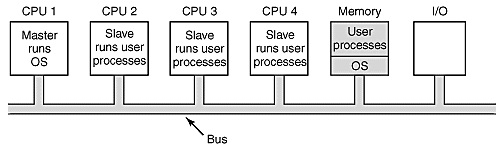
\includegraphics[scale=0.75]{Nachname/pics/assym} \cite{sureshPic}
\end{center}


\subsubsection{Symmetrisches Modell} \quad \\
Bei dem symmetrischen Modell existiert von dem Betriebssystem nur eine Kopie im Speicher, die jeder Kern 
ausführen kann. Bei Ausführung wird der entsprechende Teil des Betriebssystems in die CPU, auf der der 
Aufruf stattfand. \cite{tanenb2009} Die Systemtabellen sind ebenfalls im Speicher angelegt. \\
Daraus resultiert, dass das Bottleneck-Problem des Master-Slave-Modells umgangen wird. Ein solch verteiltes 
System bringt aber auch Probleme mit sich, sobald mehrere Teile des Systems mit gleichen oder ähnlichen 
Aufgaben auf mehreren CPUs rechnen. Ein einfacher Weg wäre das Betriebssystem durch Sperren zu 
versehen, leider führt das zu einem abgewandelten Master-Slave-Modell. \\
Da ein Betriebssystem allerdings viele voneinander unabhängige Aufgaben erfüllen muss, beispielsweise den 
Zugriff auf das Dateisystem, das Scheduling, Rechteverwaltungen und  Speicherverwaltung. Man kann das 
Betriebssystem also in solche Bereiche aufteilen und die einzelnen Bereiche durch Sperren schützen, sollten 
zwei Elemente auf den selben Speicherbereich zugreifen müssen solche Bereiche auch geschützt werden, damit 
nicht durch mehrere CPU-Prozesse eine zeitgleiche Manipulation erfolgt. Hierbei ist unter allen Umständen 
die Vermeidung von Deadlocks zu beachten. \\
\begin{center}
	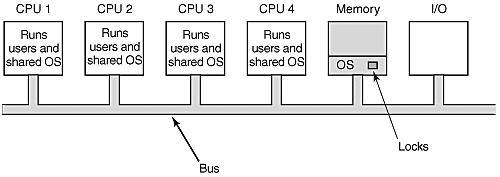
\includegraphics[scale=0.75]{Nachname/pics/symm} \cite{sureshPic}
\end{center}
\subsection{Synchronisation}
Sobald ein System über mehrere Recheneinheiten verfügt, wird die Frage des Speicherzugriffs an kritischen
Sektoren, also des Reader-, Writer-Problems immer wichtiger. Bei einer einzelnen CPU kann diese Frage durch
Interrupts gelöst werden. Interrupts können als das Sperren der normalen Ausführungsreihenfolge zu Gunsten
eines einzelnen Prozesses beschrieben werden. \\
Leider gelten Interrupts nur CPU-weit, also können Prozesse anderer CPUs den Speicherbereich, der vom 
unterbrechendem Prozess als kritisch betrachtet wird, nutzen und somit Probleme hervorrufen. \\
Eine Möglichkeit dies zu umgehen wäre ein globales Mutex-Protokoll. Ein Mutex ist ein binäres 
Sperrprotokoll, basierend auf den Stati gesperrt und nicht gesperrt. Wenn ein Prozess einen Speicherbereich 
sichern will setzt er den Mutex für diesen Speicherbereich auf gesperrt und wird ausgeführt. Will nun ein 
weiterer Prozess auf den selben Bereich schreiben, muss er warten bis der Mutex auf nicht gesperrt gesetzt 
wird. Ähnlich verhält es sich, wenn ein Prozess einen gesperrten Bereich lesen will, dies verhindert dirty 
reads. Somit werden die entsprechenden Prozessabschnitte atomarisiert. \\
Problematisch ist der Moment, in dem 2 Prozessoren gleichzeitig den selben, nicht gesperrten Abschnitt 
beschreiben wollen. Da es sich bei Mutexen um ein Frage-Antwort-Protokoll handelt, bekommen beide Prozesse 
über den gleichen Bus ein Signal, dass die Bereitschaft beschrieben zu werden zeigt. Um dieses Problem zu 
umgehen wird der entsprechende Bus durch die anfragende CPU gesperrt.

\subsection{Multiprozessor-Scheduling}
Beim Multiprozessor-Scheduling werden die Scheduling-Strategien auf mehrere CPUs angewandt und somit eine 
zusätzliche Dimension, die Entscheidung auf welcher CPU ein Prozess berechnet werden soll, zum Scheduling 
hinzugefügt. Wenn den Kernen die Existenz von Threads bekannt sind, ist es auch möglich einen Prozess auf 
mehrere Kerne aufzuteilen. \cite{tanenb2009} \\
Für Echtzeitscheduling gilt hierbei für Schedularisierbarkeit die Formel: \[\sum\limits_{i=1}^{n}\frac{C_i}
{P_i} \leq MP\] wobei \(MP\) der Anzahl der Prozessoren entspricht, die verschiedenen Prozesse werden also 
implizit auf die Prozessoren aufgeteilt, ansonsten gelten die selben Prinzipien, wie bei Ein-Kern-
Betriebssystemen für den Schedularisierbarkeitstest.
\\

\section{Fazit}
Dank Multiprogrammierbarkeit nimmt die Notwendigkeit zur Aufteilung der Hardwareressourcen zu. Besonders 
die Prozessoren als zentrale Rechenelemente müssen mit vielen Aufgaben zur gleichen Zeit zurecht kommen, 
somit behält das Prozessscheduling seine Bedeutung im Themenbereich Nebenläufigkeit. \\
Auch die zunehmende Anzahl von einzelnen Ressourcen pro System hat über die Zeit zugenommen, was die breite 
Fächerung von Nebenläufigkeiten allein im Bereich der CPU die von Betriebssystemen geregelt werden müssen 
unterstreicht. \\
Aufgrund der beobachtbaren Zunahme der Softwarekomplexität ist eine Abnahme des Stellenwertes von 
Nebenläufigkeit, der Ressourcenkonkurrenz, des Schedulings nicht wahrscheinlich.
\\ \\ \\ \\ \\ \\ \\ \\ \\ \\ \\ \\ \\ \\ \\ \\ \\ \\ \\ \\ \\ \\ \\ \\ \\ \\ \\


\pagebreak
\nocite{*}
%ESDes
%ScheThAlgSys
%OSThreePieces2014
%tanenb2009
%$